\documentclass[a4paper]{article}
\usepackage[utf8]{inputenc}
\usepackage[russian]{babel}
\usepackage{listings}
\usepackage[a4paper]{geometry}
\usepackage{indentfirst}
\usepackage{graphicx}
\usepackage{caption}
\usepackage{float}
\usepackage{amssymb}
\usepackage{physics}
\usepackage{subfig}

\begin{document}

\title{Лабораторная работа 7 по курсу <<Вычислительные задачи прикладной математики>>. \\Отчёт.}
\author{Владислав Соврасов\\ 2-о-051318}
\date{}
\maketitle

\section{Сравнение наивного и Gillespie методов для моделирования процесса случайного распада вещества}

%Naive solver time, 1d  0.025703907012939453
%Gillespie time, 1d  0.003153562545776367

\begin{figure}[H]
	\center
	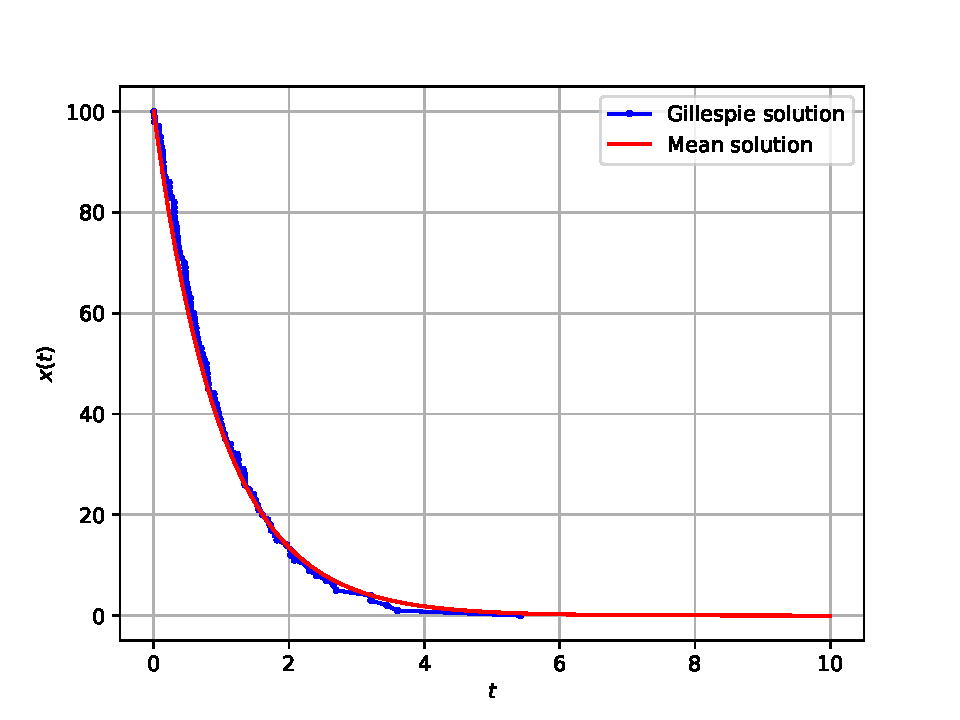
\includegraphics[width=0.75\textwidth]{../pictures/lab7_eq_1.pdf}
	\caption{Решения уравнения распада, полученные различными методами}
	\label{fig:1d_decay}
\end{figure}

\begin{figure}[H]
	\center
  \subfloat[]{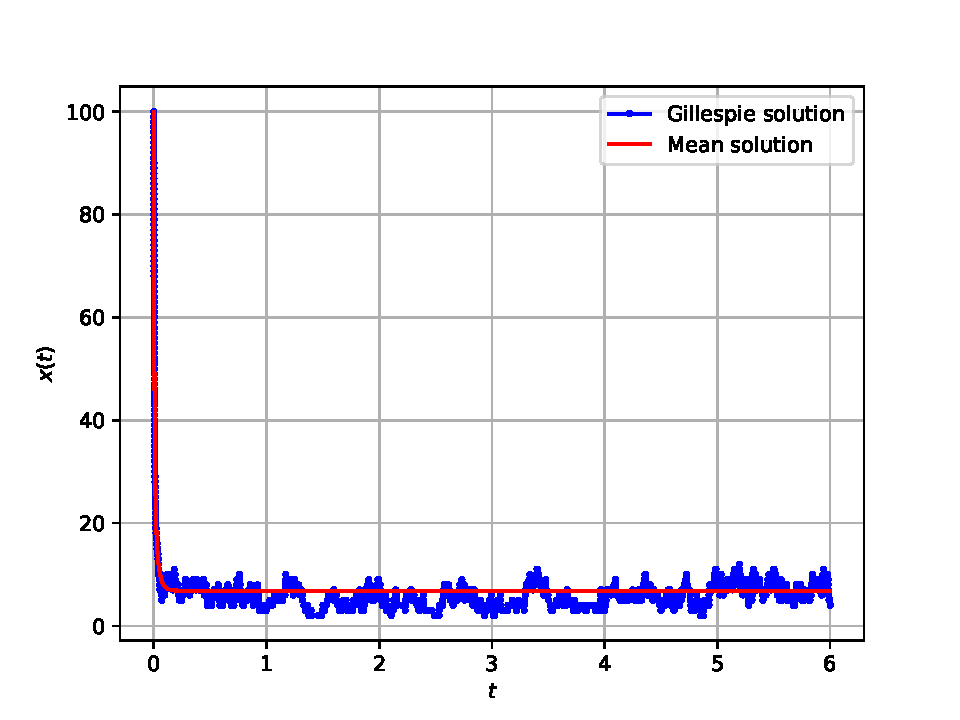
\includegraphics[width=0.6\textwidth]{../pictures/lab7_eq_2_1.pdf}\label{fig:2d_1}}
	\subfloat[]{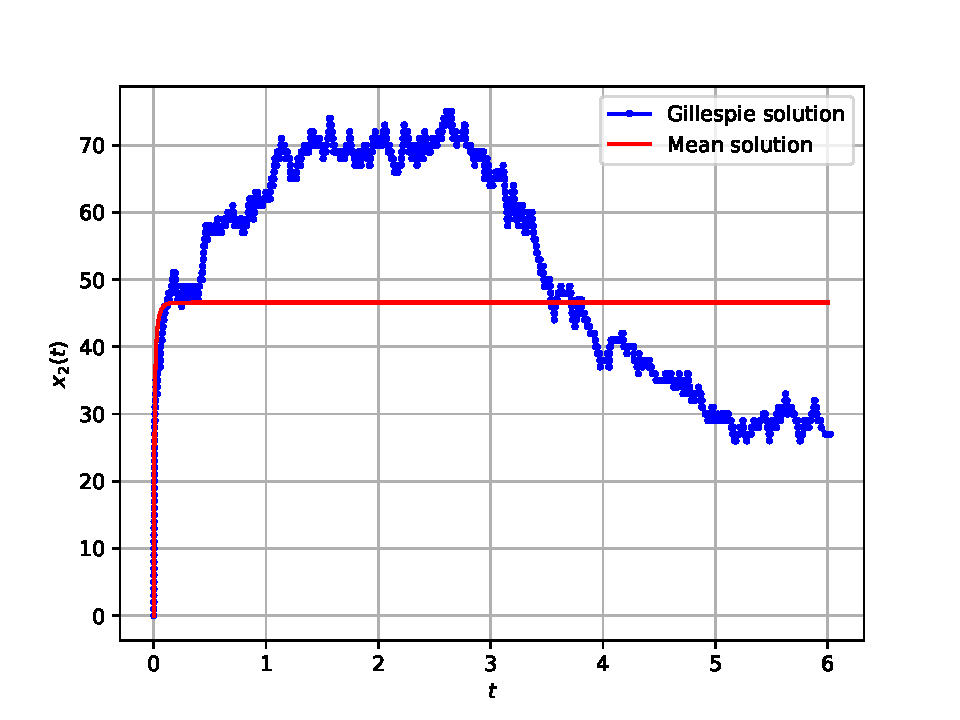
\includegraphics[width=0.6\textwidth]{../pictures/lab7_eq_2_2.pdf}\label{fig:2d_2}}
	\caption{Решения двухмерной системы уравнений}
\end{figure}

\section{Исходный код}
\lstinputlisting[language=Python, numbers=left]{../scripts/lab7.py}

\end{document}
